\chapter{Spektrale Graphentheorie}

\section{Einführung}

\begin{itemize}
  \item \emph{Spektrum} eines Graphen zur Untersuchung seiner Eigenschaften
  \item \emph{algebraische} oder \emph{spektrale Graphentheorie} genannt
\end{itemize}

Algebraische Methoden sind sehr effektiv bei Graphen, die regulär und symmetrisch sind.

\subsection{Eigenwerte, Eigenvektoren und Eigenfunktionen}

$\ma{M}\gls{eiv} = \gls{lambda}\gls{eiv}$\\
Zu einem Eigenwert $\gls{lambda}$ gibt es unendlich viele (skalierte) Eigenvektoren \gls{eiv}.
Wir definieren einen Eigenvektor \gls{eiv} dann eindeutig über $\left\|\gls{eiv}\right\|_2 = 1$.
Wenn \ma{M} symmetrisch ist und $\gls{eiv}_1$ und $\gls{eiv}_2$ zwei unterschiedliche Eigenvektoren, dann gilt $\gls{eiv}_1 \gls{ortho} \gls{eiv}_2$.
Jede symmetrische Matrix $\in \gls{R}^{n \times n}$ hat genau $n$ Eigenwerte mit $\gls{lambda}_1 \leq \cdots \leq \gls{lambda}_n$

Wir definieren $\gls{Lambda} = \gls{diag}\left(\left[\gls{lambda}_1, \ldots, \gls{lambda}_n\right]\right)$.
Wir definieren die orthogonale Matrix $\gls{Eiv} = \left[\gls{eiv}_1, \ldots, \gls{eiv}_n\right]$.
Dann gilt $\ma{M}\gls{Eiv} = \gls{Eiv}\gls{Lambda}$.
Daraus folgt sofort
\begin{equation}
  \ma{M} = \ma{M}\gls{Eiv}\gls{Eiv}^{\top} = \gls{Eiv}\gls{Lambda}\gls{Eiv}^{\top}
\end{equation}

mit $\gls{Eiv}\gls{Eiv}^{\top} = \gls{I}$.

\todo{Eigenfunktionen, brauch ich überhaupt?}

\subsection{Der Laplacian und seine Eigenwerte}

\begin{itemize}
  \item diskrete Analogie des $\nabla^2$ Operators
  \item man nimmt eine Funktion und approximiert sie mit Hilfe eines Graphen, so dass Knoten, die dichter beieinander liegen eine größere zweite Ableitung besitzen.
\end{itemize}

Der nicht-normalisierte Laplacian \gls{L} eines Graphen \gls{G} ist definiert als $\gls{L} = \gls{D} - \gls{A}$~\cite{Chung}.
Er wird auch oft kombinatorischer Laplacian genannt.
Der normalisierte Laplacian \gls{Lnorm} ist definiert als $\gls{Lnorm} = \gls{D}^{-\frac{1}{2}} \gls{L} \gls{D}^{-\frac{1}{2}}$~\cite{Chung}.
\todo{wie nennt man ihn auch?}
Es gilt die Konvention, dass ${\left(\gls{D}^{-\frac{1}{2}}\right)}_{ii} = 0$ falls $\gls{D}_{ii} = 0$ (im Falle von isolierten Knoten)
Für verbundene Graphen gilt weiterhin $\gls{Lnorm} = \gls{I} - \gls{D}^{-\frac{1}{2}} \gls{A} \gls{D}^{-\frac{1}{2}}$~\cite{Chung}.
Jeder Eintrag der Diagonalen von \gls{Lnorm} ist damit $1$.
\gls{Lnorm} ist weiterhin symmetrisch, das wäre bei einer Normierung der Form $\gls{D}^{-1}\gls{L}$ nicht der Fall.

\gls{L} und \gls{Lnorm} sind keine ähnlichen Matrizen.
Insbesondere sind ihre Eigenvektoren unterschiedlich.
Die Nutzung von \gls{L} oder \gls{Lnorm} ist damit abhängig von dem Problem, welches man betrachtet.~\cite{Hammond}.

Wir schreiben \gls{Lboth} wenn die Wahl des Laplacian \gls{L} oder \gls{Lnorm} irrelevant ist.

\subsection{Visuelle Interpretation des Laplacian}

$\nabla^2 f = \nabla \cdot \nabla f$

Die Divergenz eines Vektorfeldes ist ein Skalarfeld, das an jedem Punkt angibt, wie sehr die Vektoren in einer kleinen Umgebung des Punktes auseinanderstreben.

The Laplace operator measures how much a function differs at a point from the average of the values of the function over small spheres centered at that point. As it turns out, the Laplacian of a graph does something completely analogous: namely, it measures how much a function on a graph differs at a vertex from the average of the values of the function over the neighbors of the vertex.

Im $n$-dimensionalen euklischen Raum
\begin{equation}
  \nabla^2f = \sum_{i=1}^n \frac{\partial^2f}{\partial x^2_k}
\end{equation}
in einer Dimension reduziert sich der Laplace-Operator auf die zweite Ableitung $\nabla^2 f = f^{\prime\prime}$.

Der \emph{diskrete Laplace-Operator} ist eine Analogie zum diskreten Laplace-Operator, der finite Differenzen $x \pm h$ zur Approximation von $\nabla^2 f$ nutzt
\todo{Laplace-Operator}
\todo{diskreter Laplace-Operator} Approximation des Laplace-Operators für finite Elemente

Sei $f \colon \gls{V} \to \gls{R}$ eine Funktion auf den Knoten eines Graphen.
$f$ kann ebenso als Vektor $\ve{f} \in \gls{R}^n$ betrachtet werden mit der Ordnung der Knoten, die die Adjazenzmatrix vorgibt.

Dann gilt für \gls{Lboth}, dass
\begin{equation}
  {\left(\gls{Lboth}\ve{f}\right)}_i = \sum^n_{\substack{j=0\\j \neq i}} -\gls{Lboth}_{ij} \left(\ve{f}_i - \ve{f}_j\right)
\end{equation}

Für einen Graphen, der ein reguläres Gitter aufspannt mit gleichen Kantengewichten $\frac{1}{h^2} \in \gls{R}$ gilt für einen Knoten an Position $\left(x, y\right)$:
Abusing the index notation
\begin{equation}
  {\left(\gls{L}\ve{f}\right)}_{x,y} = \frac{4\ve{f}_{x,y} - \ve{f}_{x+1,y} - \ve{f}_{x-1,y} - \ve{f}_{x,y+1} - \ve{f}_{x,y-1}}{h^2}
\end{equation}
beschreibt die \emph{5-Punkte-Stern} Approximation $-\nabla^2 f$.
mit $\nabla^2 f$ definiert auf den fünf Punkten $\left\{\left(x,y\right), \left(x+h,y\right), \left(x-h,y\right), \left(x,y+h\right),\left(x,y-h\right)\right\}$.
\begin{equation}
  \gls{Lboth}f \approx - \nabla^2 f
\end{equation}

\todo{vertauschen, erst beispiel auf gitter, dann analog zu graphen gitter}

Damit kann der Graph Laplacian als eine Generalisierung des diskreten Laplacian auf einem Gitter verstanden werden.

Eigenwerte und Eigenvektoren werden benutzt, um zu verstehen was passiert, wenn wir einen Operator (hier \gls{Lboth}) mehrfach auf einen Vektor $\ve{x}$ anwenden (hier Merkmal auf den Knoten).

Wir können \ve{x} als Linearkombination der \emph{Eigenbasis} schreiben mit
\begin{equation}
  \ve{x} = \sum_i c_i \gls{eiv}_i
\end{equation}
und berechnen dann
\begin{equation}
  \gls{Lboth}^k \ve{x} = \sum_i c_i \gls{Lboth}^k \gls{eiv}_i = \sum_i = c_i \gls{lambda}_i \gls{Lboth}^{k-1} \gls{eiv}_i = \sum_i c_i \gls{lambda}_i^k \gls{eiv}_i
\end{equation}
Wenn wir einen Operator haben, der einen Graphen beschreibt, dann können Eigenschaften dieses Operators und damit des Graphen selber durch dessen Eigenwerte und Eigenvektoren beschrieben werden.

\subsection{Eigenschaften}

Jede Reihen- und Spaltensumme von $\gls{Lboth}$ ist $0$, d.h.\ $\sum_i \gls{Lboth}_{ij} = 0$ und $\sum_i \gls{Lboth}_{ji} = 0$ für alle $i \in \left\{1, \ldots, n\right\}$.

$\gls{Lboth} \in \gls{R}^{n \times n}$ hat genau $n$ Eigenwerte ${\left\{\gls{lambda}_i\right\}}_{i = 1}^n$, wobei die Eigenwerte für gewöhnlich aufsteigend sortiert werden, d.h.\ $\gls{lambda}_i \leq \gls{lambda}_{i+1}$.

\gls{Lboth} ist eine symmetrische reelle Matrix, d.h.\ insbesondere liegen ihre Eigenwerte $\gls{lambda}_i$ in $\gls{R+}$.
Damit ist \gls{Lboth} positiv semidefinit, d.h. $\ve{x}^{\top}\gls{Lboth}\ve{x} \geq 0$ für alle $\ve{x} \in \gls{R}^n$.\todo{quelle}

Anzahl der Eigenvektoren gleich Null ist die Anzahl an Komponenten, die ein Graph besitzt.
Insbesondere gilt $\gls{lambda}_1 = 0$, da ${\left[1, \ldots, 1\right]}^{\top} \in \gls{R}^n$ Eigenvektor von \gls{Lboth}\todo{quelle, warum gilt das}\\
$0 = \gls{lambda}_1 < \gls{lambda}_2 \leq \cdots \leq \gls{lambda}_n$ wenn Graph verbunden.\todo{quelle}\\
Für einen Graphen \gls{G} definieren wir $\gls{lambda}_{\gls{G}} := \gls{lambda}_2$ und $\gls{lambda}_{\max} := \gls{lambda}_n$
Für \gls{Lnorm} gilt $\gls{lambda}_{\max} \leq 2$\todo{quelle}

Für $\gls{Lboth}^{k}$ mit $k \in \gls{N}$ gilt ${\left(\gls{Lboth}^k\right)}_{ij} = 0$ genau dann, wenn $\gls{s}\left(v_i, v_j\right) > k$~\cite{Hammond}.
Damit beschreibt $\gls{Lboth}^k$ bildlich gesprochen die Menge an Knoten, die maximal $k$ Kanten entfernt liegen.

Eine Verschrumpfung eines Graphen \gls{G} kann beschrieben werden über zwei verschiedene Knoten $u$ und $v$ zu einem neuen Knoten $v^*$ mit
\begin{align}
  \gls{w}\left(x,v^*\right) &= \gls{w}\left(x, u\right) + \gls{w}\left(x, v\right)\\
  \gls{w}\left(v^*, v^*\right) &= \gls{w}\left(u, u\right) + \gls{w}\left(v, v\right) + 2\gls{w}\left(u,v\right)
\end{align}

Für einen Graphen \gls{G} gilt für einen Graphen $H$, der aus \gls{G} verkleinert wurde,
\begin{equation}
  \gls{lambda}_{\gls{G}} \leq \gls{lambda}_H
\end{equation}

\section{Graph-Fourier-Transformation}

Directly extending this construction to arbitrary weighted graphs is problematic, as it is unclear
how to define scaling and translation on an irregular graph.
We approach this problem by working in the spectral graph domain, i.e.\ the space of eigenfunctions of the graph Laplacian \gls{Lboth}.
This tool from spectral graph theory, provides an analogue of the Fourier transform for functions on weighted graphs.

Eigenwerte werden als Frequenz aufgefasst, die das Spektrum des Graphen beschreiben.
Die Eigenvektoren beschreiben beschreiben die Signale zu den gegebenen Frequenzen.

Fourier-Transformation beschreibt die gleiche Funktion $f$, aber in einer völlig anderen Domäne.
Nicht in der Vertex-Domäne, sondern in der Spectrum-Domäne, d.h.\ auf Basis der Eigenwerte.

Ein Signal in der Fourier-Transformierten wird daher beschrieben durch den \glqq{}Anteil\grqq\ oder die Amplituden der Eigenwerte des Graphen.\todo{das stimmt so nicht}

Fourier Transformation:
\todo{warum kann man die Fourier Transformation so definieren?}
\begin{equation}
  \ve{\hat f}_i = \hat f\left(\gls{lambda}_i\right) = \sum_{j=1}^{n} f\left(v_j\right) {\left(\gls{eiv}_i\right)}_j = \sum_{j=1}^{n} \ve{f}_j {\left(\gls{eiv}_i\right)}_j
\end{equation}
oder in Matrixschreibweise
\begin{equation}
  \ve{\hat f} = \gls{Eiv}^{\top}\ve{f}
\end{equation}

Inverse Fourier Transformation
\begin{equation}
  \ve{f}_i = f\left(v_i\right) = \sum_{j=1}^n \hat f\left(\gls{lambda}_j\right) {\left(\gls{eiv}_j\right)}_i = \sum_{j=1}^n \ve{\hat f}_j {\left(\gls{eiv}_j\right)}_i
\end{equation}
oder in Matrisschreibweise
\begin{equation}
  \ve{f} = \gls{Eiv}\ve{\hat f}
\end{equation}

Fourier-Transformation hat gute Eigenschaften (Faltung ist reine Multiplikation)
Mittels der Fouriertransformierten kann man die Faltung zweier Funktionen als Produkt ihrer Fouriertransformierten ausdrücken.

\section{Spectral Graph Domain}

\begin{itemize}
  \item \emph{Spectral Graph Domain}: Der Raum der Eigenfunktionen von $\mathcal{L}$
  \item Analogon (Nachbildung) einer \emph{Fourier-Transformation} von Funktionen auf gewichteten Graphen
\end{itemize}

Eine beliebige Funktion $f: V \rightarrow \mathbb{R}$ kann als ein Vektor in $\mathbb{R}^n$ gesehen werden.
Dies impliziert eine Ordnung auf den Knoten.
Wir schreiben $f \in \mathbb{R}^n$ für Funktionen auf den Knoten eines Graphen und $f(m)$ für den Wert des $m$ten Knoten.

Dann gilt für eine beliebige Funktion $f \in \mathbb{R}^n$

\begin{equation}
  \mathcal{L}f(x) = \sum_{x~y} w(x, y) \cdot (f(x) - f(y))
\end{equation}

wobei die Summe über $x~y$ die Summierung über alle Knoten $y$ beschreibt, die adjazent zu $x$ sind.

Angenommen $G$ ist als ein reguläres Gitter definiert der Breite und Höhe $M$
Dann hat ein Knoten $v_{x,y}$ genau 4 Nachbarn mit Kantengewicht $\frac{1}{{(\delta w)}^2}$, bei dem $\delta w$ die euklidsche Distanz zwischen zwei Gitterpunkten beschreibt.

Für eine Funktion $f: M \times M \rightarrow \mathbb{R}$ gilt dann:

\begin{equation}
  \mathcal{L}f(x, y) = \frac{4f(x,y) - f(x+1, y) - f(x-1, y) - f(x, y+1) - f(x, y-1)}{{(\delta w)}^2}
\end{equation}

Damit kann ein Signal $f$ mit der Multiplikation mit $\mathcal{L}$ als eine Weiterpropagation von $f$ unter der Berücksichtigung der lokalen Nachbarn verstanden werden (\emph{5-point Stencil}, d.h.\ $\mathcal{L}f \approx - \nabla^2 f$).

\section{Diskrete Fourier Transformation}

$\mathcal{L}$ besitzt genau $n$ orthogonal zueinander stehende Eigenvektoren $\lbrace u_l \rbrace_{l=1}^n \in \mathbb{R}^n$.
Eigenvektoren $u_i$ sind auf $1$ normiert, d.h.\ $||u_i||_2 = 1$.
Diese werden auch \emph{Graph Fourier Modes} genannt.
Diesen sind Eigenwete $\lbrace \gls{lambda}_l \rbrace_{l=1}^n \in \mathbb{R}$ zugeordnet, die die \glqq{}Frequenzen\grqq\ bzw.\ das Spektrum des Graphen beschreiben oder visuell betrachtet die Ausdehnung des Raumes, den die Eigenvektoren aufspannen.
Bemerke dass $\gls{lambda}_0 = 0$, da für den Eigenvektor $\vec{u_0} = {(1, 1, \ldots, 1)}^T$ gilt, dass $\mathcal{L}\vec{u_0} = 0$.
$\mathcal{L}$ ist diagonalisierbar über $\mathcal{L} = U \Lambda U^T$, wobei $U = [u_1, \ldots, u_n] \in \mathbb{R}^{n \times n}$ die \emph{Fourier Basis} und $\Lambda = \text{diag}([\gls{lambda}_0, \ldots, \gls{lambda}_n]) \in \mathbb{R}^{n \times n}$.
Die \emph{Fourier Transformation} eines Signals $x \in \mathbb{R}^n$ ist dann definiert als $\hat{x} = U^{T}x$ und die Inverse als $x = U\hat{x}$.

\section{Faltung}

Wir suchen einen Operator $x *_G g$, der eine Faltung zweier Eingangssignale $x, g$ zu einem Ausgangssignal umleitet.
$x$ beschreibt dabei die Knotenattribute und $g$ die Gewichte.

\subsection{Faltung in CNNs}

In der Funktionalanalysis beschreibt die \emph{Faltung} einen mathematischen Operator, der für zwei Funktion $f$ und $g$ eine dirtte Funktion $f * g$ liefert.
Die Faltung kann als ein Produkt von Funktionen vertanden werden.

Anschaulich ist $(f * g)(x)$ der \emph{gewichtete Mittelwert} von $f$, wobei die Gewichtung durch $g$ gegeben ist.

Angenommen wir wollen über einer Matrix mit einem \emph{Filter} falten.
Sei unsere Eingangsmatrix $3 \times 4$ und unsere Filtergröße $2 \times 2$.

Dann gilt zum Beispiel für den Faltungsoperator $*$ in einem Convolutional Neural Network:

\begin{equation}
  \begin{pmatrix}
    1 & 2 & 3 & 1\\
    4 & 5 & 6 & 1\\
    7 & 8 & 9 & 1
  \end{pmatrix} * \begin{pmatrix}
    1 & 1\\
    1 & 1
  \end{pmatrix} = \begin{pmatrix}
    12 & 16 & 11\\
    24 & 28 & 17
  \end{pmatrix}
\end{equation}

$f: 3 \times 4 \rightarrow \mathbb{R}$ und $g: 2 \ times 2 \rightarrow \mathbb{R}$, dann ist $*$ definiert als

\begin{equation}
  (f * g)(x, y) = \sum_{x_i \in [x, x+1]\\y_i \in [y, y+1]} f(x_i, y_i)g(x-x_i, y-y_i)
\end{equation}

\subsection{Faltung auf Graphen}

Da wir keinen Translationsoperator auf der Domäne der Knoten $x$ beschreiben können, müssen wir unseren Faltungsoperator in der Fourier-Domäne beschreiben.
Dafür wandeln wir unsere Knotenmenge $x$ zuerst in $\hat x$ um.

Wir definieren $*_G$ in der Fouier-Domäne als

\begin{equation}
  x *_G g = U \cdot (U^T \cdot x \odot \hat g)
\end{equation}

wobei $\odot(A, B) = (a_{ij} \cdot b_{ij})$ die elementweise Multiplikation bzw.\ das \emph{Hadamard-Produkt}.

Das Hadamard-Produkt löst sich auf, wenn $\hat g$ als eine Diagonalmatrix repräsentiert wird. Dann gilt

\begin{equation}
  x *_G g = U \begin{pmatrix}
    \hat g(\gls{lambda}_0) & \cdots & 0\\
    0 & \cdots & \hat g(\gls{lambda}_n)
  \end{pmatrix}U^T x = U \hat g(\Lambda) U^T x
\end{equation}

Dann beschreibt $\hat g(\Lambda) = \text{diag}(\theta)$ eine Gewichtsfunktion mit $n$ Variablen, $\theta \in \mathbb{R}^n$.
Damit ist die Faltung bzw.\ die Gewichtung abhängig von der Input-Größe $n$, was extrem schlecht ist.

\subsection{Offene Fragen}

\begin{itemize}
  \item Wie erklärt sich noch einmal der normalisierte Laplacian?
  \item Warum wird $\hat g$ als Diagonalmatrix repräsentiert?
  \item Wie kommt die Convolution zustande mit dem $*$ Operator?
  \item Was passiert bei gerichteten Graphen???? Wir haben keinen symmetrischen und insbesondere keinen positiv definiten
\end{itemize}

\section{Chebyshev Polynome}

\section{Probleme}

Rotationsinvariant

\section{Pfadlänge}

wenn $d_G(m,n) > k$, dann ${(L^k)}_{m, n} = 0$
(normalisiert sowie unnormalisiert (siehe Wavelet Lemma 5.4))

\section{Eigenwerte und Eigenvektoren reell symmetrischer Matrizen}

$\ma{M}\gls{eiv} = \gls{lambda}\gls{eiv}$\\
Zu einem Eigenwert $\gls{lambda}$ gibt es unendlich viele (skalierte) Eigenvektoren \gls{eiv}.
Wir definieren einen Eigenvektor \gls{eiv} dann eindeutig über $\left\|\gls{eiv}\right\|_2 = 1$.
Sei \ma{M} weiterhin reell symmetrisch, d.h. $\ma{M} = \ma{M}^{\top} \in \gls{R}^{n \times n}$.
Dann gilt für zwei unterschiedliche Eigenvektoren $\gls{eiv}_1$ und $\gls{eiv}_2$, dass $\gls{eiv}_1 \gls{ortho} \gls{eiv}_2$.
\ma{M} hat dann genau $n$ reelle Eigenwerte mit ${\left\{\gls{lambda}_i\right\}}_{i=1}^n$.
Wir definieren $\gls{Lambda} = \gls{diag}\left(\left[\gls{lambda}_1, \ldots, \gls{lambda}_n\right]\right)$.

Wir definieren die orthogonale Matrix $\gls{Eiv} = \left[\gls{eiv}_1, \ldots, \gls{eiv}_n\right] \in \gls{R}^{n \times n}$.
Dann gilt $\ma{M}\gls{Eiv} = \gls{Eiv}\gls{Lambda}$.
und insbesondere ist \ma{M} diagonalisierbar über
\begin{equation}
  \ma{M} = \ma{M}\gls{Eiv}\gls{Eiv}^{\top} = \gls{Eiv}\gls{Lambda}\gls{Eiv}^{\top}
\end{equation}

mit $\gls{Eiv}\gls{Eiv}^{\top} = \gls{I}$.

Damit gilt insbesondere für symmetrisch reelle Matrizen $\ma{M}$, $k \in \gls{N}$
\begin{equation}
  \ma{M}^k = {\left(\gls{Eiv}\gls{Lambda}\gls{Eiv}^{\top}\right)}^k = \gls{Eiv}\gls{Lambda}^k\gls{Eiv}^{\top}
\end{equation}

Diesen Zusammenhang kann man sicht leicht erklären, wenn man die Potenz ausschreibt:
\begin{equation}
  {\left(\gls{Eiv}\gls{Lambda}\gls{Eiv}^{\top}\right)}^k = \gls{Eiv}\gls{Lambda}\gls{Eiv}^{\top}\gls{Eiv}\gls{Lambda}\gls{Eiv}^{\top}\prod^{k-2}_{i=1} \gls{Eiv}\gls{Lambda}\gls{Eiv}^{\top} = \gls{Eiv}\gls{Lambda}^2\gls{Eiv}^{\top} \prod^{k-2}_{i=1} \gls{Eiv}\gls{Lambda}\gls{Eiv}^{\top} = \gls{Eiv}\gls{Lambda}^k \gls{Eiv}^{\top}
\end{equation}

Falls \ma{M} weiterhin \emph{schwach diagonaldominant} ist, d.h
\begin{equation}
  \sum_{j=1}^n \left|\ma{M}_{ij}\right| \leq \left|\ma{M}\right|_{ii}
\end{equation}
für alle $i \in \left\{1, \ldots, n\right\}$ sind ihre Eigenwerte $\lambda_i \in \gls{R+}$ positiv reell und wir können auf diesen eine Ordnung definieren mit $0 \leq \gls{lambda}_1 \leq \cdots \gls{lambda}_n$.
Insbesondere ist \ma{M} dann \emph{positiv-semidefinit}, das bedeutet
\begin{equation}
  \ve{x}^{\top}\ma{M}\ve{x} \geq 0
\end{equation}

\section{Der Laplacian und seine Eigenwerte}

Der \emph{kombinatorische Laplacian} \gls{L} eines Graphen \gls{G} ist definiert als $\gls{L} = \gls{D} - \gls{A}$~\cite{Chung}.
$\gls{L}$ ist eine symmetrische Matrix.

Der \emph{normalisierte Laplacian} \gls{Lnorm} ist definiert als $\gls{Lnorm} = \gls{D}^{-\frac{1}{2}} \gls{L} \gls{D}^{-\frac{1}{2}}$~\cite{Chung}.
Es gilt die Konvention, dass ${\left(\gls{D}^{-\frac{1}{2}}\right)}_{ii} = 0$ falls $\gls{D}_{ii} = 0$ (d.h.\ $v_i$ ist isolierter Knoten)

Für verbundene Graphen gilt damit $\gls{Lnorm} = \gls{I} - \gls{D}^{-\frac{1}{2}} \gls{A} \gls{D}^{-\frac{1}{2}}$~\cite{Chung}.
Jeder Eintrag der Diagonalen von \gls{Lnorm} ist damit $1$.
\gls{Lnorm} ist weiterhin symmetrisch, das wäre bei einer Normierung der Form $\gls{D}^{-1}\gls{L}$ nicht der Fall.

\gls{L} und \gls{Lnorm} sind keine ähnlichen Matrizen.
Insbesondere sind ihre Eigenvektoren unterschiedlich.
Die Nutzung von \gls{L} oder \gls{Lnorm} ist damit abhängig von dem Problem, welches man betrachtet.~\cite{Hammond}.

Wir schreiben \gls{Lboth} wenn die Wahl des Laplacian \gls{L} oder \gls{Lnorm} irrelevant ist.

\subsection{Visuelle Interpretation des Laplacian}

\begin{itemize}
  \item diskrete Analogie des $\nabla^2$ Operators
  \item man nimmt eine Funktion und approximiert sie mit Hilfe eines Graphen, so dass Knoten, die dichter beieinander liegen eine größere zweite Ableitung besitzen.
\end{itemize}


$\nabla^2 f = \nabla \cdot \nabla f$

Die Divergenz eines Vektorfeldes ist ein Skalarfeld, das an jedem Punkt angibt, wie sehr die Vektoren in einer kleinen Umgebung des Punktes auseinanderstreben.

The Laplace operator measures how much a function differs at a point from the average of the values of the function over small spheres centered at that point. As it turns out, the Laplacian of a graph does something completely analogous: namely, it measures how much a function on a graph differs at a vertex from the average of the values of the function over the neighbors of the vertex.

Im $n$-dimensionalen euklischen Raum
\begin{equation}
  \nabla^2f = \sum_{i=1}^n \frac{\partial^2f}{\partial x^2_k}
\end{equation}
in einer Dimension reduziert sich der Laplace-Operator auf die zweite Ableitung $\nabla^2 f = f^{\prime\prime}$.

Der \emph{diskrete Laplace-Operator} ist eine Analogie zum diskreten Laplace-Operator, der finite Differenzen $x \pm h$ zur Approximation von $\nabla^2 f$ nutzt
\todo{Laplace-Operator}
\todo{diskreter Laplace-Operator} Approximation des Laplace-Operators für finite Elemente

Sei $f \colon \gls{V} \to \gls{R}$ eine Funktion auf den Knoten eines Graphen.
$f$ kann ebenso als Vektor $\ve{f} \in \gls{R}^n$ betrachtet werden mit der Ordnung der Knoten, die die Adjazenzmatrix vorgibt.

Dann gilt für \gls{Lboth}, dass
\begin{equation}
  {\left(\gls{Lboth}\ve{f}\right)}_i = \sum^n_{\substack{j=0\\j \neq i}} -\gls{Lboth}_{ij} \left(\ve{f}_i - \ve{f}_j\right)
\end{equation}

Für einen Graphen, der ein reguläres Gitter aufspannt mit gleichen Kantengewichten $\frac{1}{h^2} \in \gls{R}$ gilt für einen Knoten an Position $\left(x, y\right)$:
Abusing the index notation
\begin{equation}
  {\left(\gls{L}\ve{f}\right)}_{x,y} = \frac{4\ve{f}_{x,y} - \ve{f}_{x+1,y} - \ve{f}_{x-1,y} - \ve{f}_{x,y+1} - \ve{f}_{x,y-1}}{h^2}
\end{equation}
beschreibt die \emph{5-Punkte-Stern} Approximation $-\nabla^2 f$.
mit $\nabla^2 f$ definiert auf den fünf Punkten $\left\{\left(x,y\right), \left(x+h,y\right), \left(x-h,y\right), \left(x,y+h\right),\left(x,y-h\right)\right\}$.
\begin{equation}
  \gls{Lboth}f \approx - \nabla^2 f
\end{equation}

\todo{vertauschen, erst beispiel auf gitter, dann analog zu graphen gitter}

Damit kann der Graph Laplacian als eine Generalisierung des diskreten Laplacian auf einem Gitter verstanden werden.

Eigenwerte und Eigenvektoren werden benutzt, um zu verstehen was passiert, wenn wir einen Operator (hier \gls{Lboth}) mehrfach auf einen Vektor $\ve{x}$ anwenden (hier Merkmal auf den Knoten).

Wir können \ve{x} als Linearkombination der \emph{Eigenbasis} schreiben mit
\begin{equation}
  \ve{x} = \sum_i c_i \gls{eiv}_i
\end{equation}
und berechnen dann
\begin{equation}
  \gls{Lboth}^k \ve{x} = \sum_i c_i \gls{Lboth}^k \gls{eiv}_i = \sum_i = c_i \gls{lambda}_i \gls{Lboth}^{k-1} \gls{eiv}_i = \sum_i c_i \gls{lambda}_i^k \gls{eiv}_i
\end{equation}
Wenn wir einen Operator haben, der einen Graphen beschreibt, dann können Eigenschaften dieses Operators und damit des Graphen selber durch dessen Eigenwerte und Eigenvektoren beschrieben werden.

\subsection{Eigenschaften}

\gls{Lboth} ist eine reell symmetrische, schwach diagonaldominante Matrix und damit insbesondere positiv semidefinit.

$\gls{Lboth} \in \gls{R}^{n \times n}$ hat genau $n$ Eigenwerte ${\left\{\gls{lambda}_i\right\}}_{i = 1}^n \in \gls{R+}$ mit $\gls{lambda}_i \leq \gls{lambda}_{i+1}$.

Anzahl der Eigenvektoren gleich Null ist die Anzahl an Komponenten, die ein Graph besitzt.

Insbesondere sind jede Reihen- und Spaltensumme von $\gls{Lboth}$ ist $0$, d.h.\ $\sum_j \gls{Lboth}_{ij} = 0$ und $\sum_j \gls{Lboth}_{ji} = 0$ für alle $i \in \left\{1, \ldots, n\right\}$.
Insbesondere gilt $\gls{lambda}_1 = 0$, da $\gls{eiv}_1 = \frac{1}{\sqrt{n}}{\left[1, \ldots, 1\right]}^{\top} \in \gls{R}^n$ Eigenvektor von \gls{Lboth} mit $\gls{Lboth}\gls{eiv}_1 = 0$.\\

$0 = \gls{lambda}_1 < \gls{lambda}_2 \leq \cdots \leq \gls{lambda}_n$ wenn Graph verbunden.\todo{quelle}\\

\todo{was sagt $\gls{lambda}_2$ aus?}
Für einen Graphen \gls{G} definieren wir $\gls{lambda}_{\gls{G}} := \gls{lambda}_2$ und $\gls{lambda}_{\max} := \gls{lambda}_n$
Für \gls{Lnorm} gilt $\gls{lambda}_{\max} \leq 2$\todo{quelle}

Für $\gls{Lboth}^{k}$ mit $k \in \gls{N}$ gilt ${\left(\gls{Lboth}^k\right)}_{ij} = 0$ genau dann, wenn $\gls{s}\left(v_i, v_j\right) > k$~\cite{Hammond}.
Damit beschreibt $\gls{Lboth}^k$ bildlich gesprochen die Menge an Knoten, die maximal $k$ Kanten entfernt liegen.

Eine Verschrumpfung eines Graphen \gls{G} kann beschrieben werden über zwei verschiedene Knoten $u$ und $v$ zu einem neuen Knoten $v^*$ mit
\begin{align}
  \gls{w}\left(x,v^*\right) &= \gls{w}\left(x, u\right) + \gls{w}\left(x, v\right)\\
  \gls{w}\left(v^*, v^*\right) &= \gls{w}\left(u, u\right) + \gls{w}\left(v, v\right) + 2\gls{w}\left(u,v\right)
\end{align}

Für einen Graphen \gls{G} gilt für einen Graphen $H$, der aus \gls{G} verkleinert wurde~\cite{Chung},
\begin{equation}
  \gls{lambda}_{\gls{G}} \leq \gls{lambda}_H
\end{equation}

\section{Faltung mittels Graph-Fourier-Transformation}

\subsection{Kontinuierliche Fourier-Transformation}

kontinuierliche oder klassische Fourier-Transformation:
Konvertierung eines Signals in dessen Frequenzspektrum
Signal $f \colon \gls{R} \to \gls{R}$

Die komplexe Exponentialfunktion $\exp\left(\mathrm{i}\omega t\right)$ der Fourier-Transformation beschreibt die \emph{Eigenfunktionen} des eindimensionalen Laplace-Operators $\nabla^2$.
\todo{das verstehe ich nicht}

Die inverse Fourier-Transformation
\begin{equation}
  f\left(t\right) = \frac{1}{2\pi} \int \hat f\left(\omega\right) \exp\left(\mathrm{i}\omega t\right)\,\mathrm{d}\omega
\end{equation}
kann damit als die Ausdehnung von $f$ in Bezug auf die Eigenfunktionen des Laplace-Operators gesehen werden.

\subsection{Graph-Fourier-Transformation}

Wir können die \emph{Graph-Fourier-Transformation} analog dazu definieren.\\
Eigenwerte beschreiben die Frequenzen des Graphen.

Signal $f \colon \gls{V} \to \gls{R}$ auf Graphen\\
Signal kann ebenso als Vektor $\ve{f} \in \gls{R}^n$ aufgefasst werden (impliziert Ordnung der Knoten, ist durch Adjazenzmatrix gegeben)\todo{schon weiter oben definiert, eher in grundlagen unterbringen?}\\
\begin{equation}
  \hat f(\gls{lambda}_i) = \left\langle \ve{f}, \gls{eiv}_i \right\rangle
\end{equation}
bzw.\ als Vektor
\begin{equation}
  \ve{\hat f} = \gls{Eiv}^{\top} \ve{f}
\end{equation}

Die inverse Transformation ist dann definiert als
\begin{equation}
  f\left(v_i\right) = \sum_{j=1}^n \hat f\left(\gls{lambda}_j\right) {\left(\gls{eiv}_j\right)}_i
\end{equation}
bzw.\ als Vektor
\begin{equation}
  \ve{f} = \gls{Eiv}\ve{\hat f}
\end{equation}

\todo{parseval relation?}

Spectral Graph Domain

\begin{itemize}
  \item \emph{Spectral Graph Domain}: Der Raum der Eigenfunktionen von $\mathcal{L}$
  \item Analogon (Nachbildung) einer \emph{Fourier-Transformation} von Funktionen auf gewichteten Graphen
\end{itemize}

Das ermöglicht uns das Anwenden verschiedener Operation wie Filterung, Translation oder Faltung.\todo{quelle}

Directly extending this construction to arbitrary weighted graphs is problematic, as it is unclear
how to define scaling and translation on an irregular graph.
We approach this problem by working in the spectral graph domain, i.e.\ the space of eigenfunctions of the graph Laplacian \gls{Lboth}.
This tool from spectral graph theory, provides an analogue of the Fourier transform for functions on weighted graphs.

Eigenwerte werden als Frequenz aufgefasst, die das Spektrum des Graphen beschreiben.
Die Eigenvektoren beschreiben beschreiben die Signale zu den gegebenen Frequenzen.\todo{mmh}

Fourier-Transformation beschreibt die gleiche Funktion $f$, aber in einer völlig anderen Domäne.
Nicht in der Vertex-Domäne, sondern in der Spectrum-Domäne, d.h.\ auf Basis der Eigenwerte.

In classical Fourier analysis, the eigenvalues carry a specific notion of frequency:
for $\omega$ close
to zero (low frequencies), the associated complex exponential
eigenfunctions are smooth, slowly oscillating functions,
whereas for $\omega$ far from zero (high frequencies), the associated
complex exponential eigenfunctions oscillate much more
rapidly. In the graph setting, the graph Laplacian eigenvalues
and eigenvectors provide a similar notion of frequency. For
connected graphs, the Laplacian eigenvector u0 associated
with the eigenvalue 0 is constant and equal to 1
at each
vertex. The graph Laplacian eigenvectors associated with low
frequencies $\gls{lambda}_2$ vary slowly across the graph; i.e., if two
vertices are connected by an edge with a large weight, the
values of the eigenvector at those locations are likely to be
similar. The eigenvectors associated with larger eigenvalues
oscillate more rapidly and are more likely to have dissimilar
values on vertices connected by an edge with high weight.

Graph Fourier Transformation und ihre Inverse gibt uns die Möglichkeit, ein Signal in zwei verschiedenen Domänen zu repräsentieren, nämlich die Knotendomäne (das unveränderte Signal auf der Knotenmenge $\ve{f}$) und der spektralen Domäne (das transformierte Signal in das Spektrum des Graphen).
Signale, die im Spektrum definiert werden, werden \emph{Kernel} genannt.\todo{ok?}

Die Fourier-Transformation wird unter anderem gerne genutzt, da sie gute Eigenschaften hat.

\todo{bilder bzw.\ grafiken}

\subsection{Faltung}

Es ist schwierig, Faltung auf Graphen zu definieren (wir haben keinen Translationsoperator $\left(x - t\right)$).
In der Fourier-Domäne ist dies aber sehr einfach.

In der Signalverarbeitung versteht man unter der Frequenzfilterung die Transformation eines Signals in die Fourier-Domäne und der verstärkenden oder dämpfenden Veränderung der Amplituden der Frequenzkomponenten.

Formal betrachtet also
\begin{equation}
  \hat f_{\mathrm{out}}\left(\omega\right) = \hat f_{\mathrm{in}}\left(\omega\right)\hat g\left(\omega\right)
\end{equation}

Es lässt sich zeigen, dass die Multiplikation in der Fourier-Domäne äquivalent ist zu einer Faltung in der Zeitdomäne \todo{quelle}
\begin{equation}
  f_{\mathrm{out}}\left(t\right) = \left(f_{\mathrm{in}} \star g\right)\left(t\right)
\end{equation}

Wir können das spektrale Graphfilterung analog definieren mit
\begin{equation}
  \hat f_{\mathrm{out}}\left(\gls{lambda}_i\right) = \hat f_{\mathrm{in}}\left(\gls{lambda}_i\right)\hat g\left(\lambda_i\right)
\end{equation}

Damit entspricht die Faltung eines Signals auf einem Graphen der elementweisen Multiplikation in der Spectral Graph Domain
\begin{equation}
  \ve{f}_{\mathrm{out}} = \ve{f}_{\mathrm{in}} \star \ve{g} = \gls{Eiv}\left(\gls{Eiv}^{\top}\ve{f}_{\mathrm{in}} \gls{hadamard} \gls{Eiv}^{\top}\ve{g}\right)
\end{equation}

Das lässt sich in Matrixschreibweise (die zweite obrige Formel) umschreiben über
\begin{equation}
  \ve{\hat f}_{\mathrm{out}} = \hat g\left(\gls{Lambda}\right) \ve{\hat f}_{\mathrm{in}} = \hat g\left(\gls{Lambda}\right)\gls{Eiv}^{\top}\ve{f}_{\mathrm{in}}
\end{equation}
bzw.
\begin{equation}
  \ve{f}_{\mathrm{out}} = \gls{Eiv}\hat g\left(\gls{Lambda}\right)\gls{Eiv}^{\top}\ve{f}_{\mathrm{in}}
\end{equation}
mit $\hat g\left(\gls{Lambda}\right) = \gls{diag}\left({\left[\hat g\left(\gls{lambda}_1\right), \ldots, \hat g\left(\gls{lambda}_n\right)\right]}^{\top}\right)$

\section{Polynomielle Approximation}

\begin{itemize}
  \item not localized in Space \todo{was bedeutet das?}
  \item \todo{was bedeutet $k$-localized?}
  \item Learning Komplexität linear zu der Dimension der Daten $n$
\end{itemize}

Wenn wir $\hat g\left(\gls{lambda}_i\right)$ als ein Polynom vom Grad $k$ approximieren, d.h.\

\begin{equation}
  \hat g^{\prime}(\gls{lambda}_i) = \sum_{j=0}^k c_j \gls{lambda}_i^j
\end{equation}
bzw.
\begin{equation}
  \hat g^{\prime}\left(\gls{Lambda}\right) = \sum_{j = 0}^k c_j \gls{Lambda}^j
\end{equation}
mit Koeffizienten $c_0, \ldots, c_k \in \gls{R}$, dann lässt sich der Filterungsprozess in der Spectral Graph Domain erstaunlich gut auch in der Knotendomäne interpretieren.

Der Term $\gls{Eiv}\hat g^{\prime}\left(\gls{Lambda}\right)\gls{Eiv}^{\top}$ kann dann weiter vereinfacht werden:
\begin{equation}
  \hat g^{\prime}\left(\gls{Lboth}\right) =: \gls{Eiv}\hat g^{\prime}\left(\gls{Lambda}\right)\gls{Eiv}^{\top} = \gls{Eiv} \sum_{j=0}^k c_j \gls{Lambda}^j \gls{Eiv}^{\top} = \sum_{j=0}^k c_j \gls{Eiv}\gls{Lambda}^j\gls{Eiv}^{\top} = \sum_{j=0}^k c_j \gls{Lboth}^j
\end{equation}

Das sieht man leicht mit der Beziehung $\gls{Lboth}^k = {\left(\gls{Eiv}\gls{Lambda}\gls{Eiv}^{\top}\right)}^k = \gls{Eiv}\gls{Lambda}^k\gls{Eiv}^{\top}$.\todo{bereits weiter oben definiert}

Dann ist die Faltung definiert als
\begin{equation}
  \ve{f}_{\mathrm{out}} = \hat g^{\prime}\left(\gls{Lboth}\right)\ve{f}_{\mathrm{in}}
\end{equation}
bzw.
\begin{equation}
  f_{\mathrm{out}}\left(v_i\right) = \sum_{j=0} f_{\mathrm{in}}\left(v_j\right) {\left(\hat g^{\prime}\left(\gls{Lboth}\right)\right)}_{ij}
\end{equation}
Wir erinnern uns, dass ${\left(\gls{L}^l\right)}_{ij} = 0$, wenn die kürzeste Pfadlänge $\gls{s}\left(v_i, v_j\right) > l$ von $v_i$ zu $v_j$, d.h.\ die minimale Anzahl an Kanten, größer ist als $l$.

Damit kann die Faltung in der Knotenmenge intuitiv beschrieben werden als eine gewichtete Aufsummierung bzw.\ lineare Kombination der Knotensignale in einer $k$-lokalisierten\todo{definieren} Nachbarschaft um einen Knoten $v_i$
\begin{equation}
  f_{\mathrm{out}}\left(v_i\right) = f_{\mathrm{in}}\left(v_i\right) {\left(\hat g^{\prime}\left(\gls{Lboth}\right)\right)}_{ii} + \sum_{v_j \in \mathcal{N}\left(v_i, k\right)} f_{\mathrm{in}}\left(v_j\right) {\left(\hat g^{\prime}\left(\gls{Lboth}\right)\right)}_{ij}
\end{equation}

\subsection{Tschebyschow-Polynome}

\begin{itemize}
  \item Faltung ist sehr teuer aufgrund der Berechnungen von $\gls{Lboth}^k$
  \item \underline{Idee:} beschreibe $\hat g^{\prime}\left(\gls{Lboth}\right)$ als eine polynomielle Funktion, die rekursiv aus $\gls{Lboth}$ berechnet werden kann.
  \item Warum sollte das effizienter sein? $\Rightarrow$ $\gls{Lboth}$ ist nicht dicht besetzt, und hat nur $\left|\gls{E}\right| + n \ll n^2$ Einträge mit $n \leq \left|\gls{E}\right|$
\end{itemize}

\emph{Tschebyschow-Polynome} (engl. \emph{Chebyshev}) bezeichnen eine Menge von Polynomen $\gls{T}_n\left(x\right) \colon \gls{R} \to \gls{R}$ mit dem rekursiven Zusammenhang
\begin{equation}
  \gls{T}_n\left(x\right) = 2x \gls{T}_{n-1}\left(x\right) - \gls{T}_{n-2}\left(x\right)
\end{equation}
mit $\gls{T}_0\left(x\right) = 1$ und $\gls{T}_1\left(x\right) = x$.
Ein Tschebyschow-Polynom $\gls{T}_n$ ist ein Polynom $n$-ten Grads.

Für $x \in \left[-1, 1\right]$ gilt $\gls{T}_k\left(x\right) \in \left[-1, 1\right]$

Rescale $\gls{Lambda}$ zu $\gls{tLambda} = \frac{2}{\gls{lambda}_{\max}} \gls{Lambda} - \gls{I} \in {\left[-1, 1\right]}^{n \times n}$.\todo{warum nochmal?}

Dann ist $\gls{T}_k\left(\gls{tLambda}\right) \in {\left[-1, 1\right]}^{n \times n}$

\begin{equation}
  \hat g^{\prime}\left(\gls{Lambda}\right) = \sum_{i=0}^k c_i \gls{Lambda}^i = \sum_{i = 0}^k c^{\prime}_i \gls{T}_i \left(\gls{tLambda}\right)
\end{equation}

Analog lässt sich wiederum $\hat g^{\prime}\left(\gls{Lboth}\right)$ definieren mit
\begin{equation}
  \hat g^{\prime}\left(\gls{Lboth}\right) = \sum_{i=0}^k c^{\prime}_i \gls{T}_i\left(\gls{tLboth}\right)
\end{equation}
mit $\gls{tLboth} = \gls{Eiv}\gls{tLambda}\gls{Eiv}^{\top} = \frac{2}{\gls{lambda}_{\max}} \gls{Lboth} - \gls{I}$.

Jetzt lässt sich $\ve{f}_{\mathrm{out}} = \hat g^{\prime}\left(\gls{Lboth}\right) \ve{f}_{\mathrm{in}} = \sum_{i=0}^k c^{\prime}_i \gls{T}_i \left(\gls{tLboth}\right) \ve{f}_{\mathrm{in}}$ sehr schnell berechnen:

\begin{enumerate}
  \item berechnne $\ve{\overline{f}}_i := \gls{T}_i \left(\gls{tLboth}\right) \ve{f}_{\mathrm{in}}$ für alle $i \in \left\{ 0, 1, \ldots, k \right\}$ mit Hilfe von Rekursion:
  \begin{enumerate}
    \item $\ve{\overline{f}}_0 = \ve{f}_{\mathrm{in}}$
    \item $\ve{\overline{f}}_1 = \gls{tLboth} \ve{f}_{\mathrm{in}}$
    \item $\ve{\overline{f}}_i = 2\gls{tLboth} \ve{\overline{f}}_{i-1} - \ve{\overline{f}}_{i-2}$
  \end{enumerate}
\item berechne $\ve{f}_{\mathrm{out}} = \left[\ve{\overline{f}}_0, \ve{\overline{f}}_1, \ldots, \ve{\overline{f}}_{k} \right] \ve{c}^{\prime}$, wobei $\ve{c}^{\prime} = \left[c^{\prime}_0, \ldots, c^{\prime}_k\right] \in \gls{R}^{k+1}$
\end{enumerate}

\subsubsection{Laufzeit}

 \begin{itemize}
   \item anstatt $\gls{Lboth}^k$ zu berechnen mit Komplexität $\gls{O}\left(n^2\right)$ haben wir nur noch $k$ Matrix-Vektor-Multiplikationen mit der Matrix $\gls{tLboth}$
   \item da $\gls{Lboth}$ für große Graphen sehr dünnbesetzt ist, d.h.\ $\left|\gls{E}\right| \ll n^2$, haben wir bei Verwendung von \emph{dünnbesetzten Matrizen} nur noch eine Laufzeit von $\gls{O}\left(k\left|\gls{E}\right|\right)$~\cite{Hammond, Defferrard}
   \item für den zweiten Schritt gilt $\gls{O}\left(kn\right)$, mit $n \leq \left|\gls{E}\right|$ bedingt damit nur Schritt Eins die Laufzeit
 \end{itemize}

\chapter{Graph Convolutional Networks}

\begin{equation}
  H^{(l+1)} = f(H^{(l)}, A)
\end{equation}

\begin{equation}
  f(H^{(l)}, A) = \sigma(AH^{(l)}W^{(l)})
\end{equation}

\begin{equation}
  D_{ii} = \sum_j A_{ij}
\end{equation}

Für die Potenz $x \in \gls{R}$ einer Diagonalmatrix $D \in \gls{R}^{N \times N}$ gilt:

\begin{equation}
  D^x = \begin{pmatrix}
    d_{11} & 0 & \cdots & 0\\
    0 & d_{22} & \cdots & 0\\
    \vdots & \vdots & \ddots & \vdots\\
    0 & 0 & \cdots & d_{nn}\\
  \end{pmatrix}^x = \begin{pmatrix}
    d_{11}^x & 0 & \cdots & 0\\
    0 & d_{22}^x & \cdots & 0\\
    \vdots & \vdots & \ddots & \vdots\\
    0 & 0 & \cdots & d_{nn}^x\\
  \end{pmatrix}
\end{equation}

\section{Erweiterung für mehrere Kantenattribute}

Graph Convolutional Networks berücksichtigen nur eine Adjazenzmatrix.
Das bedeutet insbesondere, dass ein Graph nur über ein Kantenattribut verfügen kann.
Das ist für ungewichtete Graphen die Markierung einer Kante ($a_{ij} \in \lbrace 0, 1 \rbrace$) oder für gewichte Graphen das Gewicht einer Kante ($a_{ij} \in \gls{R+}$).
Eine Menge von Kantenattributen kann über mehrere Adjazenzmatrizen definiert werden.
Damit ist es ebenfalls möglich unterschiedliche Kanten für unterschiedliche Attribute zu definieren.

Eine Menge von Adjazenzmatrizen $\mathcal{A} = \lbrace A_1, A_2, \ldots, A_m \rbrace$ mit $A_i \in \gls{R}^{n \times n}$ beschreibt damit eine Menge von $m$ Graphen über der gleichen Knotenmenge $\mathcal{V}$ mit Kardinalität $n$.

$\mathcal{A} \in \gls{R}^{m \times n \times n}$ kann zu einer zweidimensionalen Matrix $A \in \gls{R}^{m \cdot n \times n}$ geglättet werden.

Dann ist $A \cdot H^{(l)} \in \gls{R}^{m \cdot n \times d}$.
Reshape zu $\gls{R}^{n \times m \cdot d}$ und Gewichtsmatrix $G \in \gls{R}^{m \cdot d \times x}$.

\subsection{Übertragung auf eingebettete Graphen}

Graphknoten haben im Allgemeinen keine Position oder Lage im Raum.
Knoten, die Regionen in einer vorhandenen Segmentierung darstellen, haben jedoch offensichtlich eine gewisse Lage im Raum, die zum Beispiel über das Zentrum der Region definiert werden kann.
Diese Information ist vorhanden und wichtig und sollte demnach auch nicht verloren gehen.
Anstatt diese lokal im Knoten zu speichern, bietet es sich eher an diese Information in den Kanten zu speichern um eine bessere Faltung zu garantieren.
Die euklische Distanz zwischen zwei benacharten Regionszentren wahrt zwar die Information der Distanz zweier Knoten zueinander, verliert aber die Information der Position zweier Knoten zueinander.
Es bietet sich daher an, die horizontalen und vertikalen Abstände in einer Koordinate an den Kanten zu speichern.
Es ist zu beachten, dass wir dadurch zu einem gerichteten Graphen übergehen, bei dem jede Kante von $v$ nach $w$ auch eine Kante von $w$ nach $v$ besitzt.

Wir haben damit zwei Adjazenzmatrizen.
Da Graph Convolutional Networks nicht mit negativen Gewichten funktionieren, müssen wir negative Koordinaten in eine weitere Adjazenzmatrix schreiben.
Wir gelangen damit zu vier Adjazenzmatrizen, die die Verbindungen von einem Knoten beschreibt, die links, rechts, oben oder unten zu ihm liegen.
Wir definieren diese Adjazenzmatrizen respektive als $A_{\text{links}}, A_{\text{rechts}}, A_{\text{oben}}$ und $A_{\text{unten}}$ (vgl. Abbildung~\ref{adjazenz_aufteilung}).
Falls eine Kante horizontal bzw.\ vertikal liegt, so definieren wir $a_{ij} = 1$ respektive für beide \glqq{}gegenüberliegenden\grqq\ Adjazenzmatrizen.

\begin{figure}
\begin{minipage}[c]{0.49\textwidth}
\begin{subfigure}[c]{\textwidth}
  \centering
  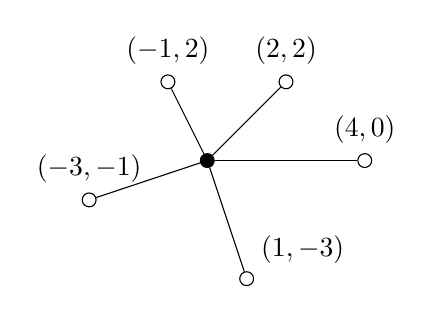
\begin{tikzpicture}
    \tikzstyle{node}=[circle,draw, minimum width=5pt, inner sep=0pt]
    \tikzstyle{root}=[fill=black]

    \node[node, root] (root) at (0,0) {};
    \node[node, label={$(-1, 2)$}] (a) at (-0.5, 1) {};
    \node[node, label={$(4, 0)$}] (b) at (2, 0) {};
    \node[node, label={$(2, 2)$}] (c) at (1, 1) {};
    \node[node, label={$(-3, -1)$}] (d) at (-1.5, -0.5) {};
    \node[node, label={50:$(1, -3)$}] (e) at (0.5, -1.5) {};

    \path (root) edge (a);
    \path (root) edge (b);
    \path (root) edge (c);
    \path (root) edge (d);
    \path (root) edge (e);
  \end{tikzpicture}
  \subcaption{Ursprüngliche Kantenattribute eines Knoten}
\end{subfigure}
\end{minipage}
\begin{minipage}[c]{0.49\textwidth}
\begin{subfigure}[c]{0.49\textwidth}
  \centering
  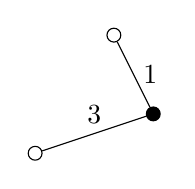
\begin{tikzpicture}
    \tikzstyle{node}=[circle,draw, minimum width=5pt, inner sep=0pt]
    \tikzstyle{root}=[fill=black]

    \node[node, root] (root) at (0,0) {};
    \node[node] (a) at (-0.5, 1) {};
    \node[node] (d) at (-1.5, -0.5) {};

    \path (root) edge[right] node {1} (a);
    \path (root) edge[above] node {3} (d);
  \end{tikzpicture}
  \subcaption{$A_{\text{links}}$}
\end{subfigure}
\begin{subfigure}[c]{0.49\textwidth}
  \centering
  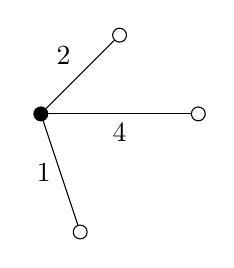
\begin{tikzpicture}
    \tikzstyle{node}=[circle,draw, minimum width=5pt, inner sep=0pt]
    \tikzstyle{root}=[fill=black]

    \node[node, root] (root) at (0,0) {};
    \node[node] (b) at (2, 0) {};
    \node[node] (c) at (1, 1) {};
    \node[node] (e) at (0.5, -1.5) {};

    \path (root) edge[below] node {4} (b);
    \path (root) edge[above left] node {2} (c);
    \path (root) edge[left] node {1} (e);
  \end{tikzpicture}
  \subcaption{$A_{\text{rechts}}$}
\end{subfigure}
\begin{subfigure}[c]{0.49\textwidth}
  \centering
  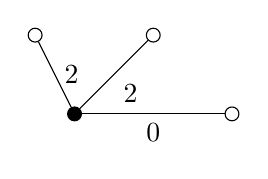
\begin{tikzpicture}
    \tikzstyle{node}=[circle,draw, minimum width=5pt, inner sep=0pt]
    \tikzstyle{root}=[fill=black]

    \node[node, root] (root) at (0,0) {};
    \node[node] (a) at (-0.5, 1) {};
    \node[node] (b) at (2, 0) {};
    \node[node] (c) at (1, 1) {};

    \path (root) edge[right] node {2} (a);
    \path (root) edge[below] node {0} (b);
    \path (root) edge[below right] node {2} (c);
  \end{tikzpicture}
  \subcaption{$A_{\text{oben}}$}
\end{subfigure}
\begin{subfigure}[c]{0.49\textwidth}
  \centering
  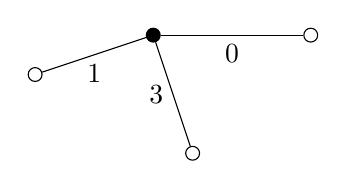
\begin{tikzpicture}
    \tikzstyle{node}=[circle,draw, minimum width=5pt, inner sep=0pt]
    \tikzstyle{root}=[fill=black]

    \node[node, root] (root) at (0,0) {};
    \node[node] (b) at (2, 0) {};
    \node[node] (d) at (-1.5, -0.5) {};
    \node[node] (e) at (0.5, -1.5) {};

    \path (root) edge[below] node {0} (b);
    \path (root) edge[below] node {1} (d);
    \path (root) edge[left] node {3} (e);
  \end{tikzpicture}
  \subcaption{$A_{\text{unten}}$}
\end{subfigure}
\end{minipage}
\caption{Aufteilung einer Adjazenzmatrix in vier räumliche Bereiche.}
\label{adjazenz_aufteilung}
\end{figure}

Kantenattribute bzw.\ Positionen von Knoten sollten skalierungsinvariant gespeichert werden.
Dafür werden die Abstände auf den Einheitskreis gemappt, wobei die längste Distanz eines Knotens auf dem Einheitskreis liegt (vgl. Abbildung~\ref{einheitskreis}).

\begin{figure}
\begin{tikzpicture}
  \draw[dashed] (0, 0) circle (4);

  \tikzstyle{node}=[circle,draw, minimum width=5pt, inner sep=0pt, fill=white]
  \tikzstyle{root}=[fill=black]

  \node[node, root] (root) at (0,0) {};
  \node[node, label={[fill=white]150:$(-1, 2) \rightarrow (-.25,.5)$}] (a) at (-1, 2) {};
  \node[node, label={[fill=white]$(4, 0) \rightarrow (1, 0)$}] (b) at (4, 0) {};
  \node[node, label={[fill=white]$(2, 2) \rightarrow (.5,.5)$}] (c) at (2, 2) {};
  \node[node, label={[fill=white]150:$(-3, -1) \rightarrow (-.75, -.25)$}] (d) at (-3, -1) {};
  \node[node, label={[fill=white]50:$(1, -3) \rightarrow (.25, -.75)$}] (e) at (1, -3) {};

  \path (root) edge (a);
  \path (root) edge (b);
  \path (root) edge (c);
  \path (root) edge (d);
  \path (root) edge (e);
\end{tikzpicture}
\caption{Abbildung der lokalen Nachbarschaftsknoten auf den Einheitskreis.}
\label{einheitskreis}
\end{figure}

Für die Anwendung auf das Graph Convolutional Network müssen die Gewichte aller Adjazenzmatrizen $a_{xij} \in [0, 1]$ invertiert werden, damit nähere Knoten einen größeren Einfluss haben.
Ebenso müssen \emph{Self Loops} für alle Knoten hinzugefügt werden.
Wir definieren unsere Adjazenzmatrix $\tilde A \in \mathbb{R}^{N \times N}$ aus einer Adjazenzmatrix $A \in \mathbb{R}^{N \times N}$ dann über

\begin{equation}
  \tilde A_{ij} = \begin{cases}
    1, & \text{falls }i=j\text{,}\\
    {(a_{ij}+1)}^{-1}, & \text{falls }a_{ij} \neq 0\text{,}\\
    0, & \text{sonst.}
  \end{cases}
\end{equation}

Dann ist $\tilde a_{ij} \in [1, 0.5]$

Diagonalmatrix ist schwierig.
Man will ja die Normalisierung damit $H^{(l)}$ nicht überskaliert.
Ich würde auch die gewichtete Matrix normalisieren.
Denke das macht Sinn.
Dann fallen die Werte ab, wenn viele Knoten weit entfernt sind.

\section{Pooling auf Graphen}
\label{pooling}

\subsection{Graphvergröberung}
\label{graphvergroeberung}

\paragraph{Clustering von Knoten}
\label{clustering_von_knoten}

\subsection{Erweiterung auf ebene Graphen}
\label{pooling_erweiterung}

\input{chapters/spectral/tangens}
\section{Beispiel}

Wir betrachten eine einfache $3 \times 3$ Adjazenzmatrix, d.h.\ $|\mathcal{V}| = n = 3$.

\begin{equation}
  A = \begin{pmatrix}
    0 & 1 & 0\\
    1 & 0 & 1\\
    0 & 1 & 0
  \end{pmatrix}
\end{equation}

mit Diagonalmatrix $D = \text{diag}(1, 2, 1)$.

Der Laplacian $\mathcal{L} = D - A$ ist dann

\begin{equation}
  \mathcal{L} = \begin{pmatrix}
    1 & -1 & 0\\
    -1 & 2 & -1\\
    0 & -1 & 1
  \end{pmatrix}
\end{equation}

Nun müssen die Eigenvektoren der Matrix und dessen Eigenwerte bestimmt werden, d.h.\ wir müssen das folgende Eigenwertproblem lösen

\begin{equation}
  \mathcal{L} \cdot \vec{u} = \lambda \cdot \vec{u}
\end{equation}

Wir erhalten $3$ Eigenvektoren und Eigenwerte mit

\begin{equation}
  \lambda_0 = 0, \vec{u}_0 = \frac{1}{\sqrt{3}} \begin{pmatrix}1\\1\\1\end{pmatrix} \approx \begin{pmatrix}0.58\\0.58\\0.58\end{pmatrix},
    \lambda_1 = 1, \vec{u}_1 = \frac{1}{\sqrt{2}} \begin{pmatrix}-1\\0\\1\end{pmatrix} \approx \begin{pmatrix}-0.71\\0\\0.71\end{pmatrix},
      \lambda_2 = 3, \vec{u}_2 = \frac{1}{\sqrt{6}} \begin{pmatrix}1\\-2\\1\end{pmatrix} \approx \begin{pmatrix}0.41\\-0.82\\0.41\end{pmatrix}
\end{equation}

Dann sind $U$, $\Lambda$ und $U^T$ definiert als

\begin{equation}
  U \approx \begin{pmatrix}
    0.58 & -0.71 & 0.41\\
    0.58 & 0 & -0.82\\
    0.58 & 0.71 & 0.41
  \end{pmatrix},
  \Lambda = \begin{pmatrix}
    0 & 0 & 0\\
    0 & 1 & 0\\
    0 & 0 & 3
  \end{pmatrix},
  U^T \approx \begin{pmatrix}
    0.58 & 0.58 & 0.58\\
    -0.71 & 0 & 0.71\\
    0.41 & -0.82 & 0.41
  \end{pmatrix}
\end{equation}

Angenommen wir haben ein Signal $x = {(100, 10, 1)}^T$, dann ist der Wert dieses Signals transformiert in die Fourier Domäne definiert als $\hat x \approx {(64.09, -70.00, 33.07)}^T$.
Führen wir $\hat x$ auf $x$ mittels $U \cdot \hat x$ zurück, erhalten wir korrekterweise $x = {(100, 10, 1)}^T$.

Es gilt $\lambda_{\max} = 3$
Jetzt ist $\mathbf{\tilde \Lambda}$ definiert als
\begin{equation}
  \mathbf{\tilde \Lambda} = \begin{bmatrix}
    -1 & 0 & 0\\
    0 & -\frac{1}{3} & 0\\
    0 & 0 & 1
  \end{bmatrix}
\end{equation}

Wir überprüfen die Approximation durch die Polynome mit $k = 2$:

\begin{equation}
  g_{\mathbf{\theta}}\left(\mathbf{\Lambda}\right) = \begin{pmatrix}
    1\\2\\3
  \end{pmatrix},
  g_{\mathbf{\theta}^{prime}} = \begin{pmatrix}
    wd
  \end{pmatrix}
\end{equation}

